\newpage

\renewcommand{\proofname}{Доведення}
\renewcommand{\chaptername}{РОЗДІЛ}
\chapter{Тренди серед мобільних фреймворків}
\label{ch1}

\section{Проблема розробки мобільних додатків}
\label{section.1.1}

React Native та Flutter - найкращі мобільні фреймворки для створення мобільних додатків для iOS та Android.
Вже кілька років спільноти розробків порівнюють ці дві платформи.

Розробка додатків з використанням оригінального фреймворку під ОС Android та iOS з використанням Android Studio та Xcode домінували у галузі мобільної розробки, поки не виникали певні проблеми.
\begin{itemize}
    \item Потреба в різних базах кодів для різних платформ (iOS та Android)
    \item Найм розробників під конкретну платформу дорого справа
    \item Витрати на розробку та обслуговування дуже високі
\end{itemize}

Щоби розв'язати проблему було впровадженне міжплатформенне рішення для мобільних розробок, такі як React Native та Flutter.

\section{Розробка крос-платформних мобільних додатків}
\label{section.1.2}
Завдяки міжплатформенній розробці підприємства та організації змогли охопити ширшу аудиторію, ефективніше та з меншими витратами.
React Native був представлений Facebook у 2015 році.
React Native - це фреймворк для мобільних додатків з відкритим кодом, який використовує React із власними можливостями платформи для розробки додатків для Android, iOS, Web та UWP.

Серед рішень, що використовують React Native: Facebook, Instagram, Tesla, Uber Eats, Discord, Wix, Walmart.

Flutter був представлений Google у травні 2017 року. Але випуск стабільної версії відбувся у грудні 2018 року.
Flutter також має відкритий вихідний код і використовується для розробки програм для Android, iOS, Linux, Mac, Windows, Google Fuchsia та веб.

Деякі програми, створені за допомогою Flutter, це: Google Ads, Alibaba.com, Realtor.com.

Оскільки Flutter та React-Native стали найгарячішою темою останніх днів та конкурентними дебатами серед спільноти розробників, багато розробників залижаються у невизначеності, визначаючи, яку платформу вибрати.

\section{Тренди}\label{section.1.3}

\begin{figure}
    \label{fig:flutter_react_trend_5_years}
    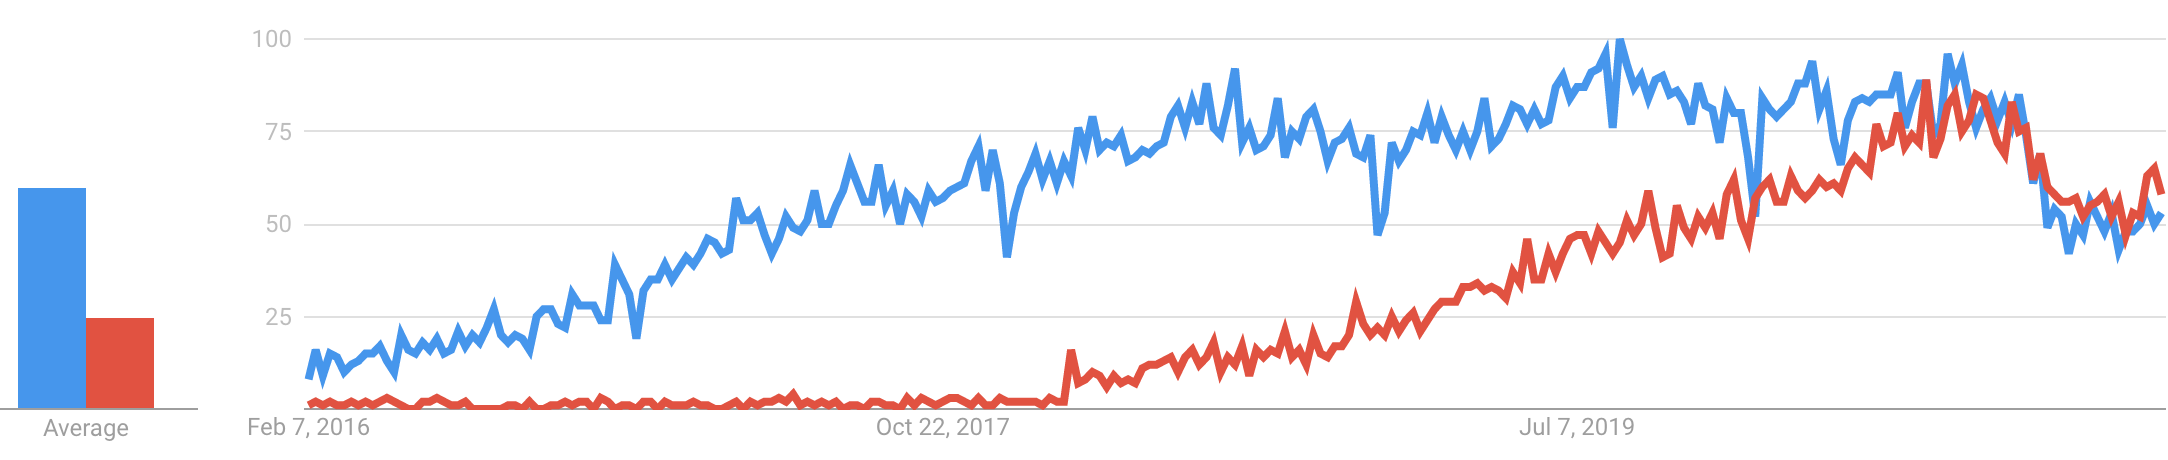
\includegraphics[scale=0.4]{flutter_react_trend_5_years.png}

    Відповідно до Google Trends за 5 років
\end{figure}

На Google Trends за останні п’ять років Flutter випередив React Native.
Але це не визначає, що Flutter - кращий варіант, ніж React Native.

Flutter був представлений зовсім недавно, тому багатьох розробників та любителів програмування рухає цікавість та інтерес до вивчення нової платформи.
Однак у галузі React Native все ще використовується розробниками, оскільки він є більш стабільним і має вищий рівень прийняття порівняно з Flutter.

\section{Мови програмування}\label{section.1.4}

Flutter використовує мову, що називається Dart. 
Це мова, яка має синтаксис, подібний до Java та Javascript.

Простим прикладом коду в Dart буде:
\begin{lstlisting}[style=light, language=Python,label={lst:vectorimg},caption=Dart Hello World]
void main () { 
  print ("Hello World!"); 
}
\end{lstlisting}

React Native використовує Javascript.
React Native побудований поверх React, який побудований на Javascript.
Тому, якщо вам доведеться вивчити React Native, вам знадобляться попередні знання Javascript.

Javascript існує довкола спільноти розробників програмного забезпечення дуже давно, і існує безліч ресурсів, на яких можна навчитися javascript.
Простим прикладом коду в javascript буде:

\begin{lstlisting}[style=light, language=Python,label={lst:vectorimg},caption=Dart Hello World]
  alert("Hello World!");
\end{lstlisting}

\section{Спільнота}\label{section.1.5}

Flutter і Dart були представлені спільноті розробників нещодавно, і порівняно, у неї менша спільнота розробників.
Google витратив багато на розробку Dart, і спільнота продовжує зростати.
Flutter має спільноти на StackOverflow, Slack та багатьох інших платформах.

React Native має більшу спільноту розробників, ніж Flutter, сприяючи його розвитку.
Спільнота Javascript є навіть більшою, ніж спільнота React Native, оскільки вона існує вже дуже давно, і допомогу можна знайти майже скрізь в Інтернеті.
Це, безумовно, пояснює, чому React Native має вищий рівень прийняття в порівнянні з Flutter.
Крім того, підтримка React, React Native та Javascript в Інтернеті є більш доступною.
Є мільйони рядків коду, які є у вільному доступі в Інтернеті, і їх можна просто «зняти» та використовувати у своїх проектах.
На сторінці спільноти React Native на їх офіційному веб-сайті вказані інші платформи, що вміщують їхні спільноти, такі як StackOverflow та Medium.

\section{Віджети інтерфейсу користувача}\label{section.1.6}
Найкраще у Dart - це те, що він постачається з повним набором віджетів інтерфейсу, які можна підняти прямо з коробки та використовувати.
В React Native, набір віджетів інтерфейсу мінімальний, і тому розробникам програмного забезпечення та програмістам доводиться звертатися до сторонніх бібліотек для віджетів інтерфейсу, і іноді їм доведеться створювати власні віджети інтерфейсу. 
